\documentclass{article}
\usepackage[left=2.5cm,right=2.5cm,top=3cm,bottom=2.75cm]{geometry}
\usepackage{gensymb}
\usepackage{graphicx}
\graphicspath{{./Documents}{./figs}}
\begin{document}
\begin{enumerate}
	\item In the given figure, PQ is tangent to the circle centred at $ \vec{O} $. If \angle{AOB} = $ 95^{\degree} $, then measure of \angle{ABQ} will be
	\begin{figure}[!h]
		\centering
		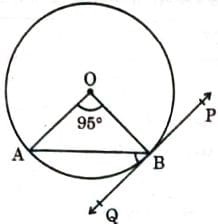
\includegraphics[scale=0.5]{1.jpg}
		\caption{Circle-1}
		\label{fig:circle}
	\end{figure}
		\begin{enumerate}
			\item $ 47.5^{\degree} $
			\item $ 42.5^{\degree} $
			\item $ 85^{\degree} $
			\item $ 95^{\degree} $
		\end{enumerate}
	\item (a) Two tangents TP and TQ are drawn to be a circle with centre $ \vec{O} $ from an external point $ \vec{T} $. Prove that \angle{PTQ} = 2\angle{OPQ}.
		\begin{figure}[!h]
			\centering
			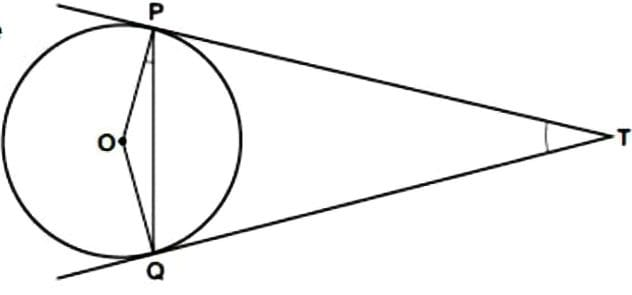
\includegraphics[scale=0.3]{2.jpg}
			\caption{Circle-2}
			\label{fig:circle}
			\textbf{OR}
		\end{figure}\\
	 (b) In the given figure, a circle is inscribed in a quadrilateral ABCD in which \angle{B} = $ 90^{\degree} $. If AD = 17 cm, AB = 20 cm and DS = 3cm, then find the radius of the circle.
		\begin{figure}[!h]
			\centering 
			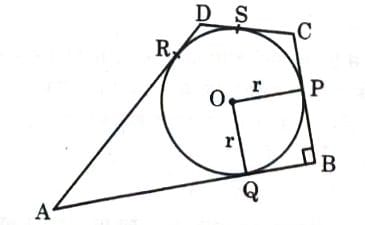
\includegraphics[scale=0.5]{3.jpg}
			\caption{Circle-3}
			\label{fig:circle}
		\end{figure}
	\item The discus throw is an event in which an athlete attempts to throw a discus. The athlete spins anti-clockwise around one and a half times through a cicrle, then releases the throw. When released, the discus travels along tangent to the circular spin orbit.
		\begin{figure}[h!]
			\centering
			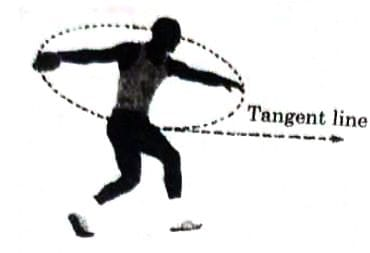
\includegraphics[scale=0.4]{4.jpg}
		\end{figure}\\
		In the given figure, AB is one such tangent to a circle of radius 75 cm. Point $ \vec{O} $ is centre of the circle and \angle{ABO} = $ 30^{\degree} $. PQ is parallel to OA.
		\begin{figure}[h!]
			\centering
			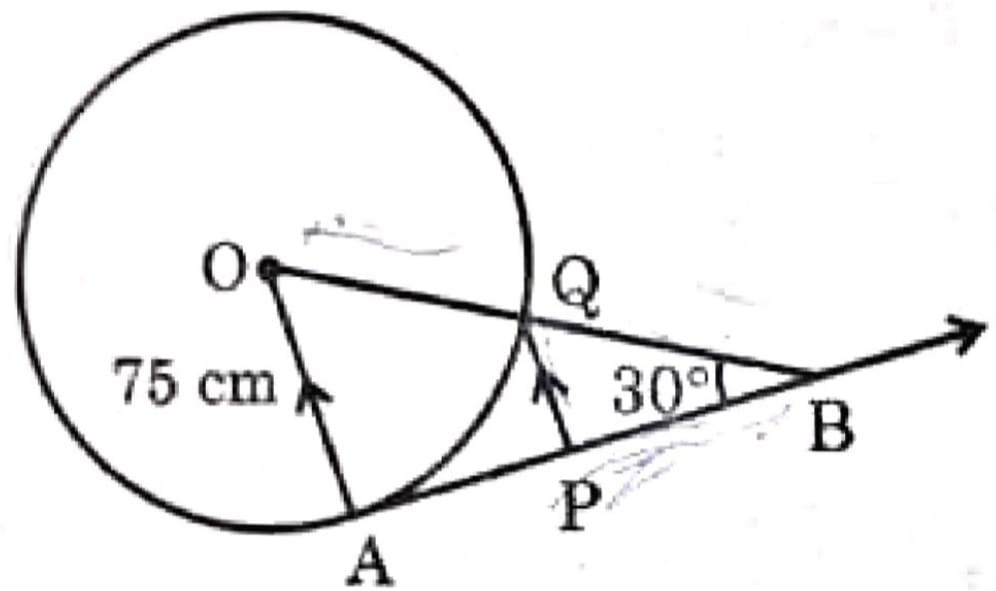
\includegraphics[scale=0.2]{5.jpg}
			\caption{Circle-4}
			\label{fig:circle}
		\end{figure}\\
		Based on above information :
		\begin{enumerate}
			\item find the length of AB.
			\item find the length of OB.
			\item find the length of AP.
			\item find the length of PQ.
		\end{enumerate}
	\item In the given figure, the quadrilateral PQRS circumscribes a circle. Here PA + CS is equal to :
		\begin{figure}[h!]
			\centering
			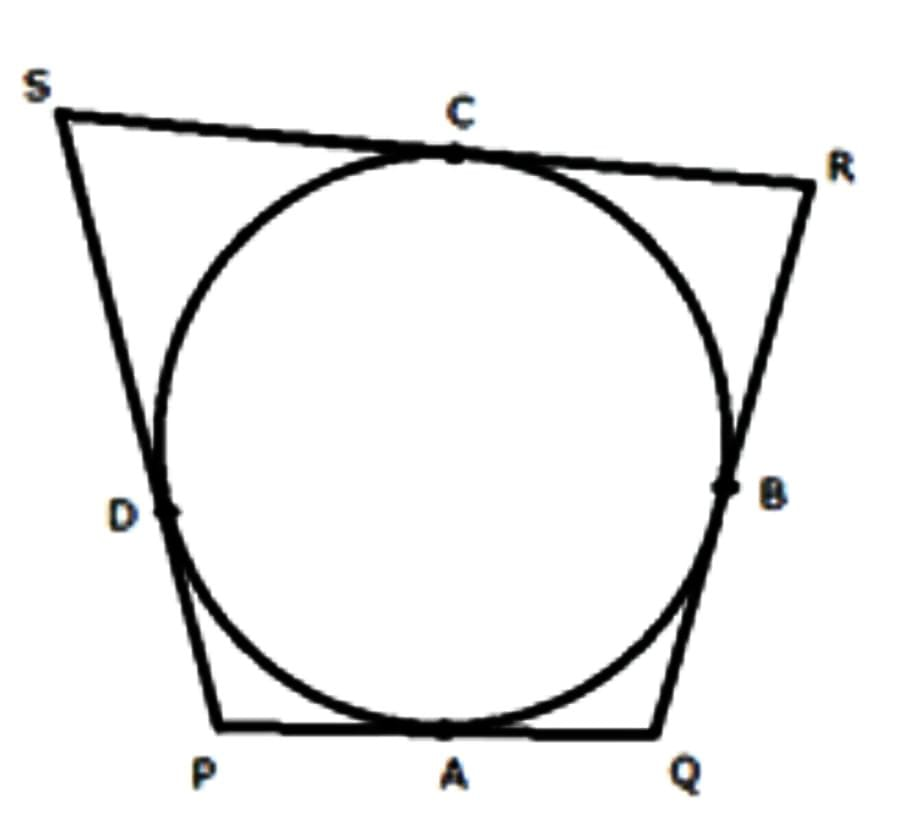
\includegraphics[scale=0.155]{6.jpg}
			\caption{Circle-5}
			\label{fig:circle}
		\end{figure}
		\begin{enumerate}
			\item QR
			\item PR
			\item PS
			\item PQ
		\end{enumerate}
	\item In the given figure, $ \vec{O} $ is the centre of the circle. AB and AC are tangents drawn to the circle from point $ \vec{A} $. If \angle{BAC} = $ 65^{\degree} $, then find the measure of \angle{BOC}.
		\begin{figure}[h!]
			\centering
			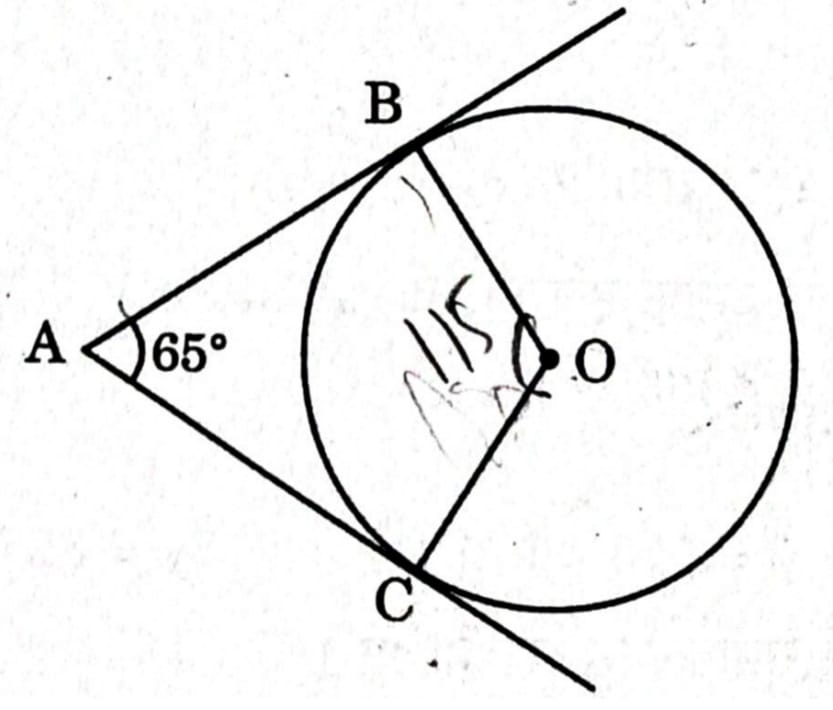
\includegraphics[scale=0.2]{7.jpg}
			\caption{Circle-6}
			\label{fig:crcle}
		\end{figure}
	\item In the given figure, $ \vec{O} $ is the centre of the circle and QPR is the tangent to it at $ \vec{P} $. Prove that \angle{QAP} + \angle{APR} = $ 90^{\degree} $.
		\begin{figure}[h!]
			\centering
			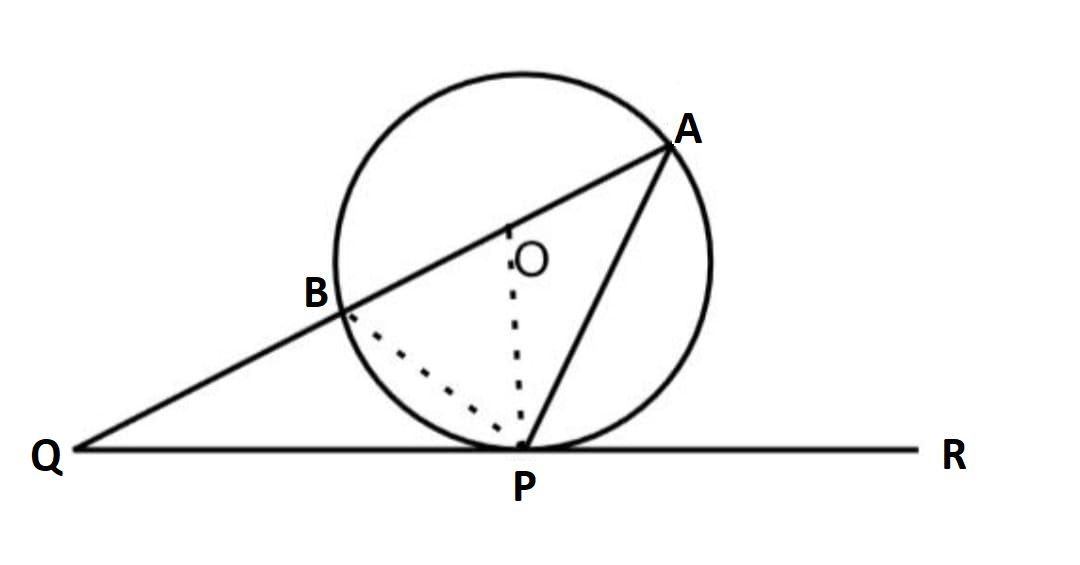
\includegraphics[scale=0.22]{8.jpg}
			\caption{Circle-7}
			\label{fig:circle}
		\end{figure}
	\item In the given figure, TA is a tangent to the circle with centre $ \vec{O} $ such that OT = 4 cm, \angle{OTA} = $ 30^{\degree} $, then length of TA is :
		\begin{figure}[h!]
			\centering
			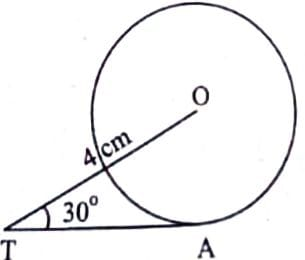
\includegraphics[scale=0.3]{9.jpg}
			\caption{Circle-8}
			\label{fig:circle}
		\end{figure}
		\begin{enumerate}
			\item $ 2\sqrt{3} $ cm
			\item 2 cm
			\item $ 2\sqrt{2} $ cm
			\item $ \sqrt{3} $ cm
		\end{enumerate}
	\item In the given figure, PT is a tangent at $ \vec{T} $ to the circle with centre $ \vec{O} $. If \angle{TPO} = $ 25^{\degree} $, then $ x $ is equal to : 
		\begin{figure}[h!]
			\centering
			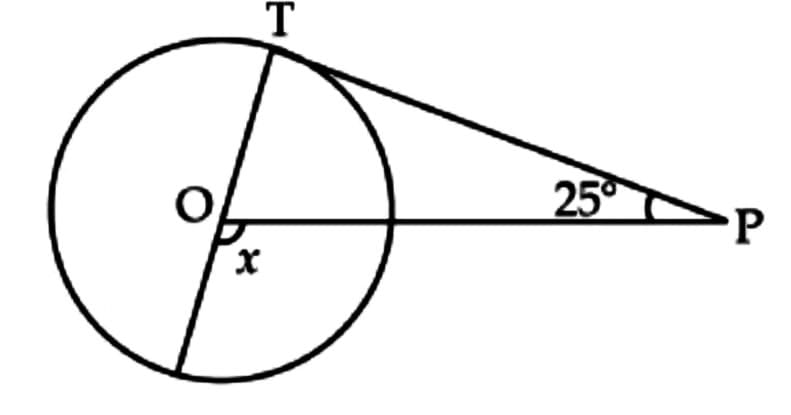
\includegraphics[scale=0.3]{10.jpg}
			\caption{Circle-9}
			\label{fig:circle}
		\end{figure}
		\begin{enumerate}
			\item $ 25^{\degree} $
			\item $ 65^{\degree} $
			\item $ 90^{\degree} $
			\item $ 115^{\degree} $
		\end{enumerate}
	\item Two concentric circles are of radii 5 cm and 3 cm. Find the length of the chord of the larger circle which touches the smaller circle.
\end{enumerate}
\end{document}
